\textbf{地址映射变换机构是将CPU送来的主存地址转换为Cache地址。}由于主存和Cache的块大小相同,块内地址都是相对于块的起始地址的偏移量(即低位地址相同),因此地址变换主要是主存块号与Cache块号之间的转换。地址变换主要有3种转换方式,即{\textbf{直接映射、全相联映射和组相联映射。}}

\textbf{1.直接映射}

图3-28为直接映射方式主存与Cache中字块的对应关系,其中Cache分为8行,主存分为256行。由于Cache被分为8块,因此在主存中可以将每8块看成一个``轮回'',这样主存就可以被分为32个``轮回''。而每个``轮回''中的第i块只能映射到Cache的第i块,类似于上面生活场景助解中的个位数为n的学生只能坐到讲台上的n号位置。如果要用一个数学表达式来表示,则很快会想到用取模来对应,如下:\\

\textbf{i=jmodC}

其中,i为Cache中的块号,j为主存中的块号,C为Cache的块数(图3-28中C等于8)。上面的公式表示将主存第j块内容复制到Cache的i块中。

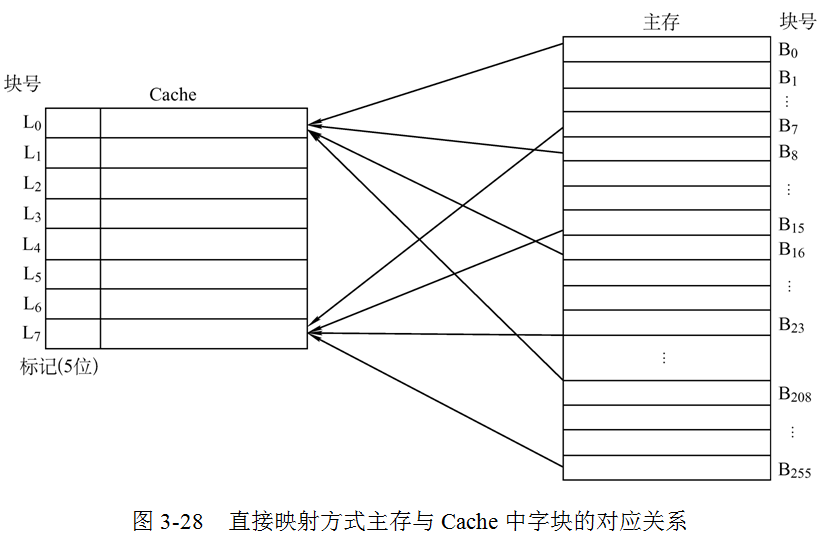
\includegraphics[width=3.69792in,height=2.43750in]{png-jpeg-pics/86BE8C5EE2A04D9E7E6BD8010BFCC50D.png}

\textbf{2.全相联映射}

图3-30为全相联映射方式主存与Cache中字块的对应关系。全相联映射允许主存中每一个字块映射到Cache中的任何一块的位置上。《计算机组成原理高分笔记》书籍里面讲过,如果是全相联映射,那么每个人需要举着两位数号码的牌子才能识别这个人。在图3-30中,主存有256块,Cache需要8位(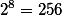
\includegraphics[width=0.64583in,height=0.15625in]{texmath/d8f4e828256})来作为标记位,这样才能识别每一个主存块。返回到图3-28,因为直接映射只需要识别每个组号即可,所以主存大小是Cache的32倍(也就是说,主存需要分为32组),即Cache需要5位来作为标记位,这样才能识别该块属于哪一组。

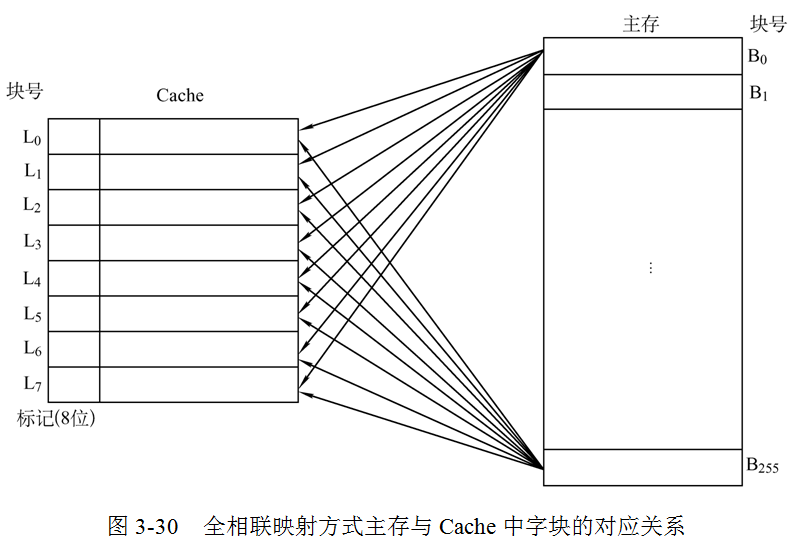
\includegraphics[width=3.69792in,height=2.54167in]{png-jpeg-pics/745532CB27FBE35BABB980604360E67C.png}

\textbf{3.组相联映射}

图3-32为组相联映射方式主存与Cache中字块的对应关系。可以看出,组相联映射是对直接映射和全相联映射进行折中的一种方式。假设把Cache分为Q组,每组有R块,现在考生需要做的事情是把组相联映射的一组看作直接映射中的一块。同理,可以得到和直接映射中一样的公式为:\textbf{i=jmodQ}

其中,i为Cache中的组号,j为主存中的块号,Q为Cache的组数(图3-32中Q等于4)。通俗地说,上面的公式就是主存第j块内容复制到Cache的i组中,至于是第i组的哪一块,那就可以随意放了。

由于Cache分为4组,因此主存的256块应该分成256/4=64个``轮回'',故需要6位tag来表示是哪一个``轮回''。

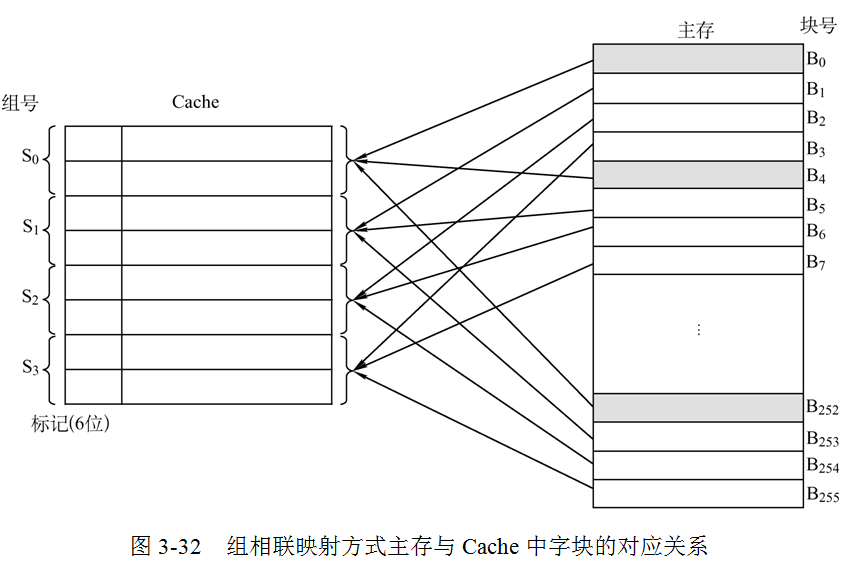
\includegraphics[width=3.69792in,height=2.45833in]{png-jpeg-pics/44C23D729B6DD2ACE9D0F48F87404873.png}

{\textbf{千万注意:组相联还有另外一种映射方式,因为12年第17题考查过,用上面的组相联无法解出此题,另一种组相联见下图:}}

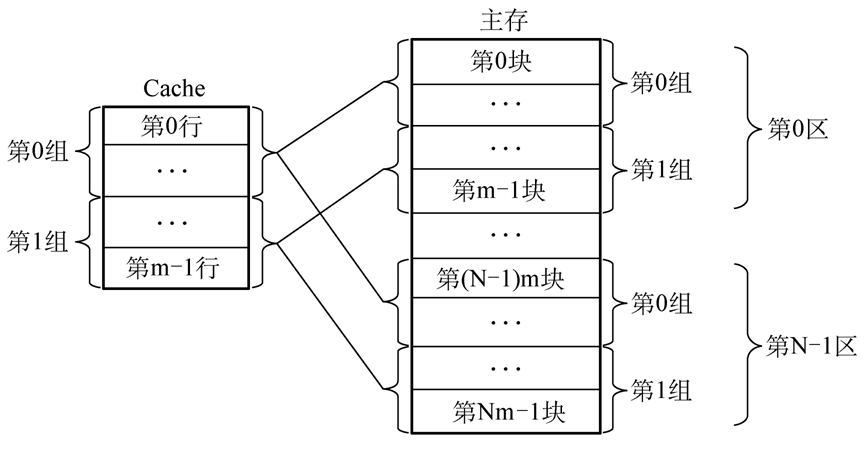
\includegraphics[width=3.52083in,height=1.84375in]{png-jpeg-pics/6C28359075578819B57C725544B589AE.png}

该方式是先将主存块按{Cache}大小分区,再将各个分区中的块进行分组,同样{Cache}内也分组,组内分块。主存中不同区的相同序号的组和{Cache}同序号的组采用直接映射(例如主存的第{X}区的第{0}组只能映射到{Cache}的第{0}组),主存和{Cache}同序号的组内各块采用全相联映射,不同序号的组没有映射关系。{}
